\documentclass[../../guia1.tex]{subfiles}
\usepackage{subfig}
\usepackage{float}
\begin{document}
\section*{Ejercicio 9}
Llamando a $x(n)=X(nT)$ y $y(n)=Y(nT)$, se obtiene la siguiente ecuación en diferencias. 
\begin{equation}
y(n)=\frac{1}{2} x(n-2) + \alpha y(n-1) + \beta y(n-2)  
\end{equation}

\subsection{a}
Siendo $\alpha = 1$ y $\beta = -\frac{1}{2}$ se simulo la respuesta al escalón y al impulso.
\begin{figure}[H]
 \centering
  \subfloat[Respuesta al escalón]{
   \label{f:ejaesc}
    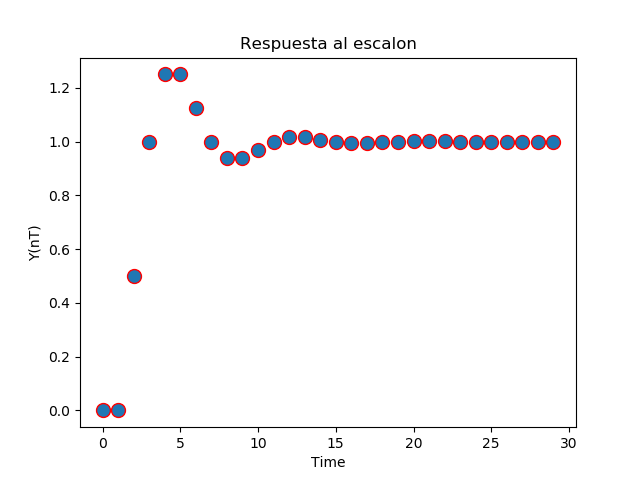
\includegraphics[width=0.6\textwidth]{figures/a-escalon.png}}
  \subfloat[Respuesta al impulso]{
   \label{f:ejaimp}
    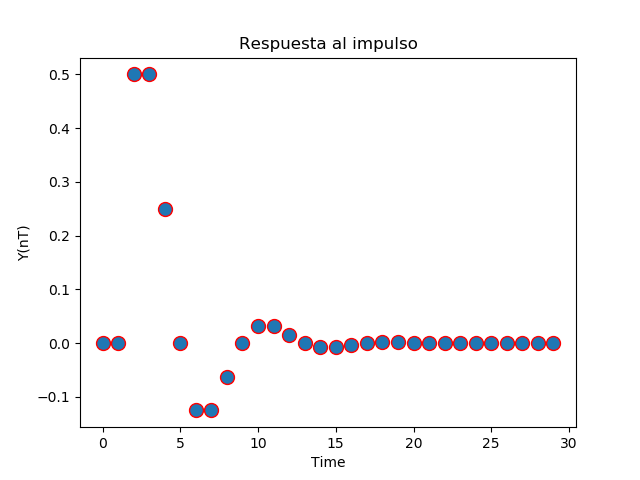
\includegraphics[width=0.6\textwidth]{figures/a-impulso.png}}

 \caption{Gráficos de la simulación de las respuesta al impulso y al escalón}
 \label{f:eja}
\end{figure}
De la simulación se obtuvo que la frecuencia de oscilación en función de $nT$ es $f= \frac{1}{8}$.
\subsection{b}
Siendo $\alpha = \frac{1}{2}$ y $\beta = -\frac{1}{8}$ se simulo la respuesta al escalón y al impulso.
\begin{figure}[H]
 \centering
  \subfloat[Respuesta al escalón]{
   \label{f:ejbesc}
    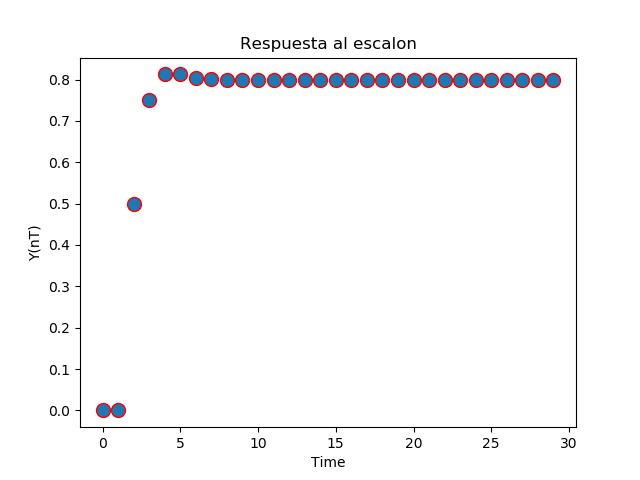
\includegraphics[width=0.6\textwidth]{figures/b-escalon.png}}
  \subfloat[Respuesta al impulso]{
   \label{f:ejbimp}
    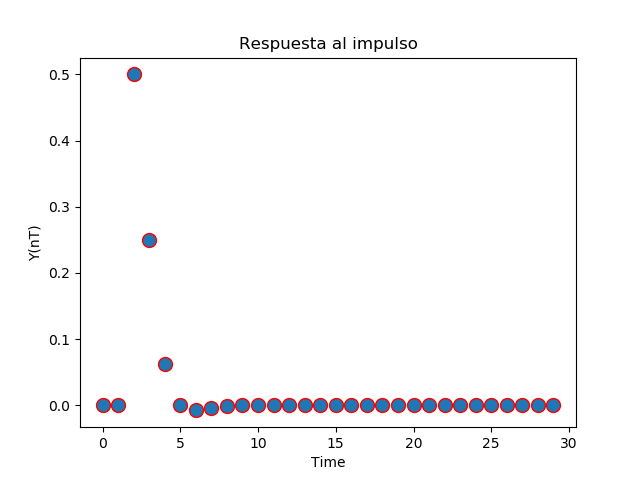
\includegraphics[width=0.6\textwidth]{figures/b-impulso.png}}

 \caption{Gráficos de la simulación de las respuesta al impulso y al escalón}
 \label{f:ejb}
\end{figure}

\subsection{c}
Siendo $\alpha = 1$ y $\beta = -\frac{1}{2}$ se simulo la respuesta al escalón y al impulso.
\begin{figure}[H]
 \centering
  \subfloat[Respuesta al escalón]{
   \label{f:ejcesc}
    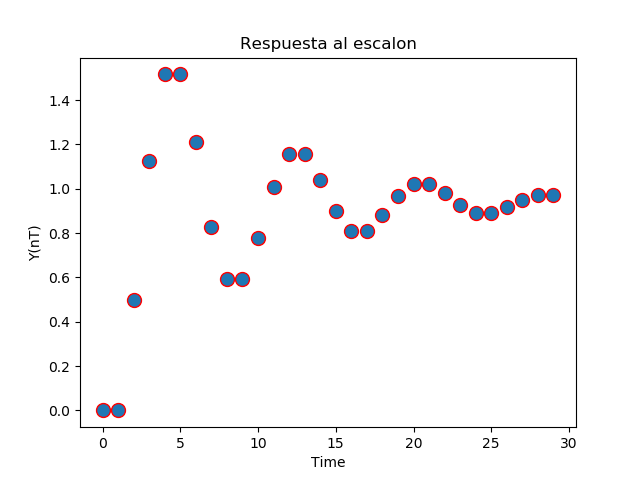
\includegraphics[width=0.6\textwidth]{figures/c-escalon.png}}
  \subfloat[Respuesta al impulso]{
   \label{f:ejcimp}
    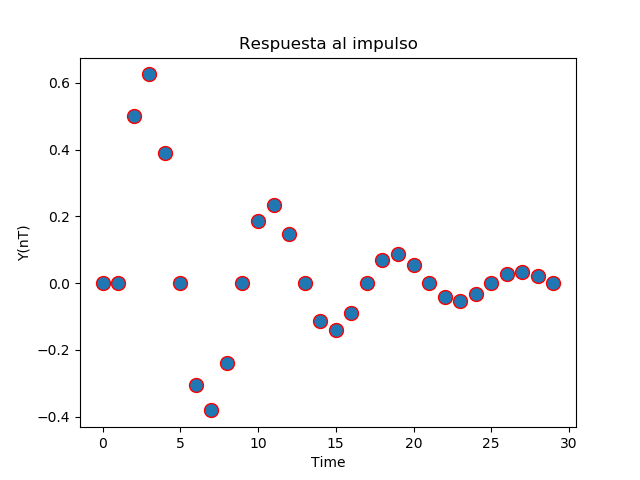
\includegraphics[width=0.6\textwidth]{figures/c-impulso.png}}

 \caption{Gráficos de la simulación de las respuesta al impulso y al escalón}
 \label{f:ejc}
\end{figure}
De la simulación se obtuvo que la frecuencia de oscilación en función de $nT$ es $f= \frac{1}{7}$
\subsection{Análisis de resultados}
Como se observa las respuesta del sistema, con los parámetros de los casos $a$ y $c$, corresponde a un sistema subamortiguado. En el caso $a$ corresponde a un sistema subamortiguado con un factor de amortiguamiento mayor que el caso $c$.
\par El caso de $c$ corresponde a un sistema críticamente amortiguado.






\end{document}
